\section{Resumen de la especificación de la NoC}
\label{sec:especificacion}

La NoC de este proyecto cuenta con las siguientes características:

\begin{itemize}[noitemsep]
    \item \textbf{Topología} en \textit{malla} de altura y ancho parametrizables.
    \item \textbf{Enlaces} \textit{full-dúplex}.
    \item Algoritmo de \textbf{encaminamiento} en \textit{Orden Dimensional} (DOR), siendo este determinista y mínimo.
    \item \textbf{Direccionamiento} mediante una tupla con las \textit{coordenadas absolutas} del dispositivo.
    \item \textbf{Conmutación} de circuitos segmentada usando \textit{flits} enviados en serie.
    \item \textbf{Arbitraje} \textit{round-robin}.
    \item Cada \textit{flit} se manda en paralelo usando un \textit{bus}.
    \item Sistema de \textbf{paquetes} con tres tipos de \textit{flits}: cabecera, datos y cola.
\end{itemize}

A nivel usuario, para poder crear dispositivos que hagan uso de la red, también deben tenerse en cuenta la \hyperref[subsec:codificacion_flits]{codificación de los flits~(\ref{subsec:codificacion_flits})} y el \hyperref[subsec:noc_protocolo]{protocolo de comunicación~(\ref{subsec:noc_protocolo})}.

\subsection{Codificación de los flits}
\label{subsec:codificacion_flits}

De un flit de tamaño \textit{FLIT\_WIDTH}, los dos primeros bits han sido reservados para un enumerado \textit{e\_flit} que representa el tipo de flit, pudiendo ser cabecera (\textit{HEADER}), datos (\textit{DATA}) o cola (\textit{TAIL}). Dependiendo del tipo de flit, podemos distinguir las siguientes responsabilidades y formatos:

\begin{description}[noitemsep]
    \item [Cabecera] Se encarga de establecer el camino virtual, por lo que contiene la dirección destino del paquete. Los bits que no tienen ningún uso especificado pueden usarse para transmitir información si es necesario.
    % Debido a que la conmutación de circuitos está segmentada, es necesario retransmitir la cabecera hasta que recibamos una señal de que se ha establecido el camino virtual.
    \item [Datos] Podemos enviar tantos flits de datos como sea necesario, pero se recomienda minimizar el tamaño del paquete para evitar la \textit{inanición} de otros paquetes de la red, pues al usar conmutación de circuitos los canales usados quedan reservados mientras se envia el paquete. Si descontamos los dos bits del enumerado, tenemos \textit{FLIT\_DATA\_WIDTH} bits para enviar información.
    \item [Cola] La única diferencia con los flits de tipo \textit{DATA} es que, cuando un nodo recibe un flit de cola, este debe liberar los recursos reservados para la conexión. Por lo tanto, solo se enviará un flit de cola al final del paquete.
\end{description}

Podemos ver una representación visual del formato de los flits en la figura \ref{fig:flits_format}.

\begin{figure}[h]
    \centering
    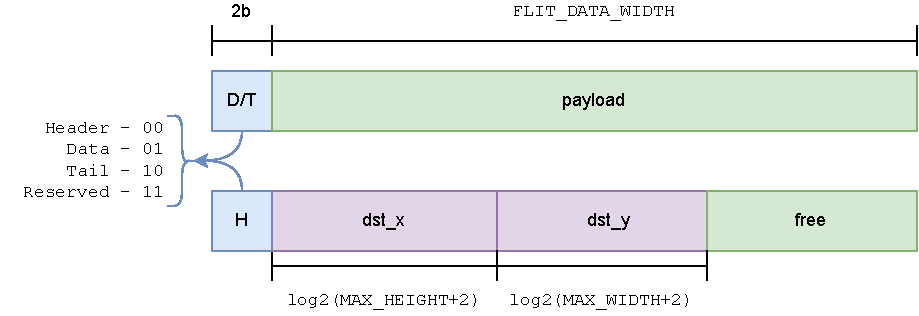
\includegraphics{images/diagrams/flit_format.drawio.pdf}
    \caption[Formato de los flits de la red]{Formato de los flits de la red. Arriba el formato de los flits de tipo datos/cola y abajo el formato de los flits cabecera.}
    \label{fig:flits_format}
\end{figure}

\subsection{Protocolo de comunicación}
\label{subsec:noc_protocolo}

En esta sección se especifica el sistema de reglas que deben seguir los usuarios de la red para transmitir y recibir información satisfactoriamente. Pueden verse ejemplos de implementación y máquinas de estado en las subsecciones \hyperref[subsec:emisor]{\ref{subsec:emisor}~\nameref{subsec:emisor}} y \hyperref[subsec:receptor]{\ref{subsec:receptor} \nameref{subsec:receptor}}.

En la comunicación entre nodos, junto al flit se envía una señal de control \textit{enable} y se recibe una respuesta \textit{ack}:
\begin{itemize}[noitemsep]
    \item \textbf{\textit{enable}}: indica al siguiente nodo que el bus del flit contiene información y es válida.
    \item \textbf{\textit{ack}}: indica al nodo anterior que se ha establecido un camino virtual y puede comenzar el envío de datos.
\end{itemize}

Usando estas dos señales y el bus de flit, la comunicación según si queremos emitir o recibir datos sería la siguiente:

\subsubsection{Emisión}

Para establecer una conexión es necesario crear una cabecera indicando la dirección de destino con el formato estipulado en el apartado anterior. A continuación, habilitamos el enlace poniendo la señal \textit{enable} a 1, y continuamos repitiendo el flit cabecera mientras se reserva el camino completo hasta recibir la señal \textit{ack}; que indica que se ha establecido el camino virtual.

Desde este momento, la señal \textit{ack} se mantendrá a 1 y podemos enviar tantos flits de tipo \textit{DATA} como sea necesario. Cuando deseemos mandar los últimos datos y liberar los recursos, mandaremos un flit de tipo \textit{TAIL}, finalizando la conexión.

\subsubsection{Recepción}

Si podemos recibir paquetes, es necesario establecer la señal \textit{ack} a 1. Cuando vayamos a recibir un paquete se habilitará la señal de entrada \textit{enable} a la vez que recibimos una cabecera. Esta cabecera podemos descartarla o almacenarla si los bits libres tienen datos de nuestro interés. Durante varios ciclos recibiremos de nuevo esta cabecera con exactamente los mismos datos, por lo que debemos descartarla hasta recibir un flit de tipo \textit{DATA}.

Los siguientes bits serán de tipo \textit{DATA} o \textit{TAIL} y contendrán la información del paquete, por lo que los procesaremos como sea necesario. Finalmente, recibiremos un flit de cola que indicará el fin de la conexión.
